\documentclass[../main.tex]{subfiles}

\begin{document}
\chapter{Results and Discussion}
\label{cha:Results}

\begin{itemize}
    \item list assumptsion
    \begin{itemize}
        \item that over rl training is a good measure of skill
        \item that win-rate is a measure of skill?
    \end{itemize}
    \item list limitations
    \begin{itemize}
        \item 
    \end{itemize}
\end{itemize}

\subsection{The effect of going first}
\begin{table}[]
    \centering
    \begin{tabular}{@{}llll@{}}
                 & Random & Novice & Intermediate \\
    Random       & 0.0655 (\minus0.0019) & 0.0186 (\pos0.0035) & 0.0111 (\pos0.0000)  \\
    Novice       & 0.9414 (\minus0.0003) & 0.5149 (\pos0.0352) & 0.3421 (\pos0.0190)  \\
    Intermediate & 0.9865 (\pos0.0023)   & 0.6921 (\pos0.0175) & 0.5206 (\pos0.0253)    
    \end{tabular}
    \caption{Win-rate matrix for rule based agents when player 0 is fixed as the starting player. Averaged over 10000 games per pairing. Row vs. Column, the agent in the row is goes first. Increase over \autoref{tab:rules-winrates} shown in brackets.}
    \label{tab:rule-wr-going-first}
\end{table}


\begin{figure}
    \centering
    \begin{subfigure}[t]{0.49\textwidth}
        \centering
        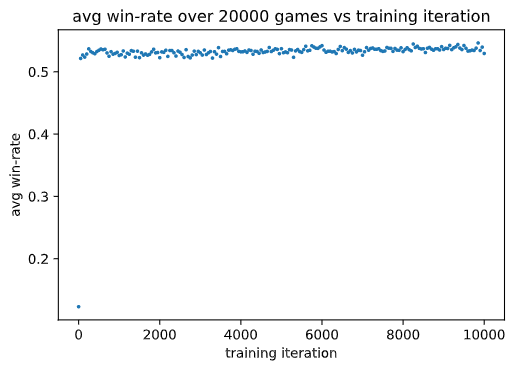
\includegraphics[width=\textwidth,keepaspectratio]{images/results/going_first_over_time.png}
        \caption{Win rate vs Training Iteration in self play when the agent going first is fixed. Every 100th training iteration using 50000.}
        \label{fig:win-rate-going-first}
    \end{subfigure}
    \hfill
    \begin{subfigure}[t]{0.49\textwidth}
        \centering
        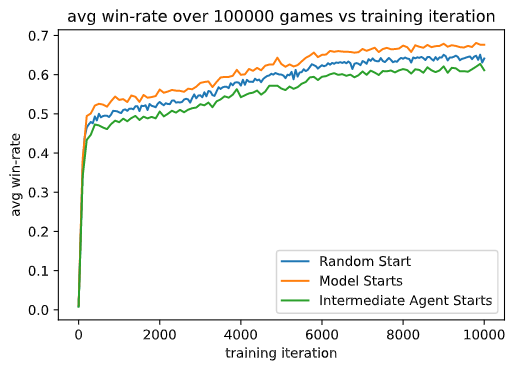
\includegraphics[width=\textwidth,keepaspectratio]{images/results/winrate_vs_int_going_first.png}
        \caption{Win-rate for the model verses the intermediate agent. }
        \label{fig:win-rate-vs-int-going-first}
    \end{subfigure}
    \caption{Going first over training iteration}
    \label{fig:going-first-over-time}
\end{figure}

\subsection{The effect of starting hands}

\subsubsection{specific score}

\begin{figure}
    \centering
    \begin{subfigure}[t]{0.49\textwidth}
        \centering
        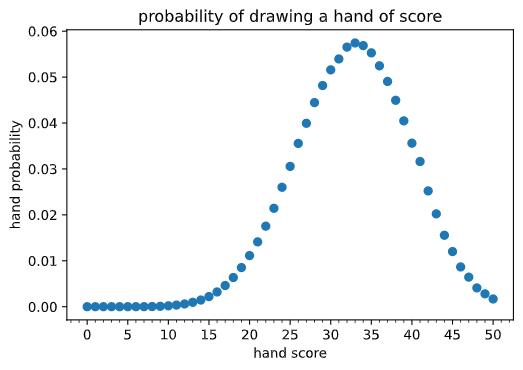
\includegraphics[width=\textwidth,keepaspectratio]{images/results/handscores.png}
        \caption{Frequency of 5 card hand combinations which score. Note that the lowest possible hand score is 6 (4 aces and a two).}
        \label{fig:startinghand-probs}
    \end{subfigure}
    \hfill
    \begin{subfigure}[t]{0.49\textwidth}
        \centering
        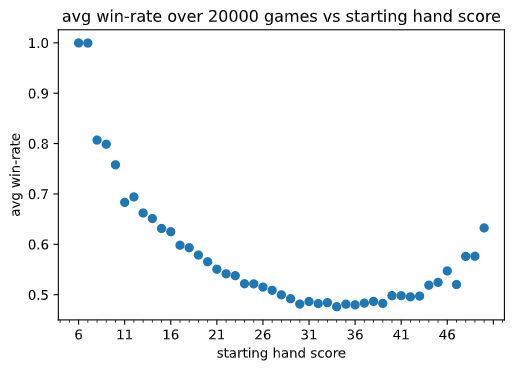
\includegraphics[width=\textwidth,keepaspectratio]{images/results/winrate_handscore.png}
        \caption{Win-rate for given starting hand score.}
        \label{fig:startinghand-winrates}
    \end{subfigure}
    \caption{Hand score results.}
    \label{fig:handscores}
\end{figure}

\subsubsection{specific class}

\begin{figure}
    \centering
    \begin{subfigure}[t]{0.49\textwidth}
        \centering
        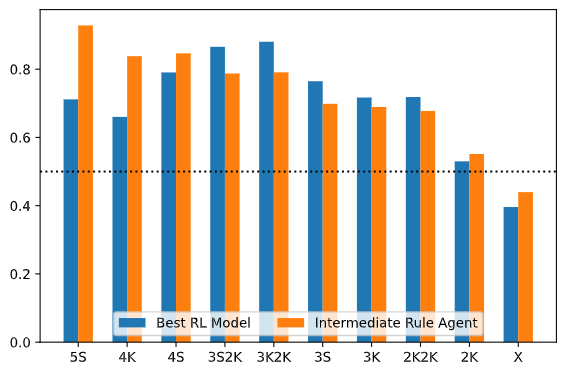
\includegraphics[width=\textwidth,keepaspectratio]{images/results/handclasses.png}
        \caption{Win rates for each handclass. Agents playing against them selves.}
        \label{fig:handclass-vs-self}
    \end{subfigure}
    \hfill
    \begin{subfigure}[t]{0.49\textwidth}
        \centering
        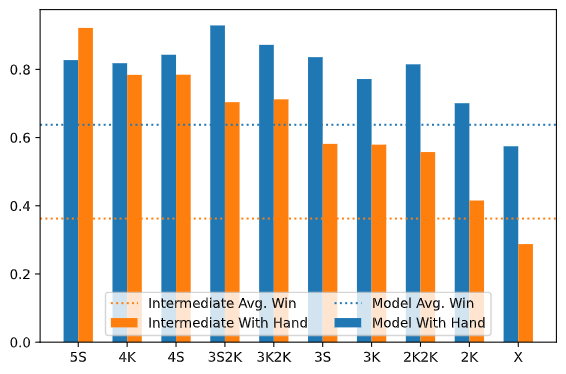
\includegraphics[width=\textwidth,keepaspectratio]{images/results/handclasses_model_vs_rules.png}
        \caption{Hand class win rates for Model vs Intermediate. Along with the base line win-rate for each (random hands).}
        \label{fig:handclass-int-vs-model}
    \end{subfigure}
    \label{fig:handclass-winrates}
    \caption{Win rates for different hand classes. Uses the intermediate rule agent and the 10,000th iteration of the RL model. Averaged over 100,000 games. The opponent's starting hand is sampled from the deck after generating the starting hand of the given class.}
\end{figure}

\begin{figure}
    \centering
    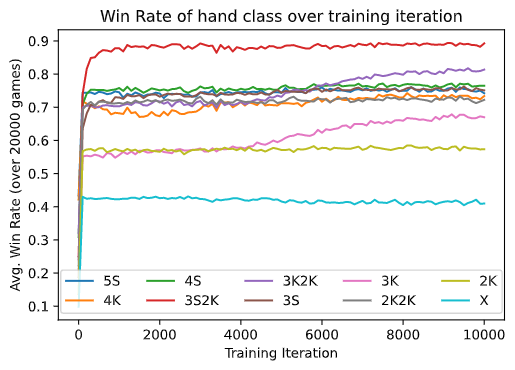
\includegraphics[width=\textwidth,keepaspectratio]{images/results/handclassovertime.png}
    \caption{Win-rate for given class over training iterations.}
    \label{fig:handclass-overtime}
\end{figure}

\end{document}